\documentclass[12pt,oneside]{book}
\usepackage{geometry}                		% See geometry.pdf to learn the layout options. There are lots.
\geometry{a4paper}                   			% ... or a4paper or a5paper or ... 
%\geometry{landscape}                		% Activate for for rotated page geometry
%\usepackage[parfill]{parskip}    		% Activate to begin paragraphs with an empty line rather than an indent
\usepackage{graphicx}				% Use pdf, png, jpg, or epsß with pdflatex; use eps in DVI mode
								% TeX will automatically convert eps --> pdf in pdflatex		
\usepackage{amssymb}

\usepackage[spanish]{babel}			% Permite que partes automáticas del documento aparezcan en castellano.
\usepackage[utf8]{inputenc}			% Permite escribir tildes y otros caracteres directamente en el .tex
\usepackage[T1]{fontenc}				% Asegura que el documento resultante use caracteres de una fuente apropiada.

\usepackage{hyperref}				% Permite poner urls y links dentro del documento

\title{Mi Juego Favorito}
\author{Javier Tibau}
%\date{}							% Activate to display a given date or no date

\begin{document}
\maketitle
\tableofcontents

\chapter{Introducción}
El libro a continuación es creado como una herramienta para el desarrollo de habilidades de edición colaborativa de documentos de texto plano. La herramienta que habilita dicha colaboración, en este taller, es Git pero podría ser reemplazada por otros sistemas de versionamiento.

\chapter{Los Juegos}

\include{juegos/Buscaminas}
\include{juegos/Dota2}
\include{juegos/Zelda}
include{juegos/TempleRun}
\section{Resident Evil}

\begin{figure}[htbp]
\begin{center}
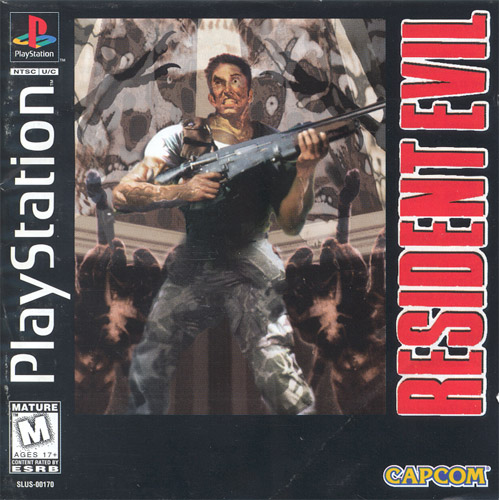
\includegraphics[width=.35\textwidth]{./imagenes/resident_evil1.jpg}
\caption{Resident Evil}
\label{Resident Evil}
\end{center}
\end{figure}
Una extraña ola de asesinatos empiezan a ocurrir en las montañas Arklay a las afueras de Racoon City.  Es entonces que la noche del 24 de julio de 1998 el departamento de policia de Racoon City envia al equipo Bravo del gurpo especial S.T.A.R.S. (Special Tactics And Rescue Service) a investigar. Al poco tiempo se pierde el contacto con el equipo Bravo y se envia al equipo Alpha a continuar la investigacion y encontrar al equipo Bravo. Al llegar son atacados por una especie de perros zombies y son obligados a refugiarse en una mansion cercana. Es Aqui Donde comienza la pesadilla de los S.T.A.R.S. por sobrevivir ya que la mansion es un centro secreto de desarrollo de armas biologicas, y los miembros de S.T.A.R.S. han sido engañados para probar una nueva arma denominada Virus-T la cual es capaz de reviir el tejido muerto a nivel celular. En Resident Evil\footnote{\url{http://www.residentevilcenter.net/residentevil.html}} entramos en la piel de los miembros del equipo Alpha de S.T.A.R.S. Chris Redfield o Jill Valentine los cuales se enfrentaran a monstruos creados con el virus-T tales como zombies y demas criaturas; con municion limitada y su sentido de supervivencia.

\subsubsection{¿Por qué es uno de mis juegos favoritos?}
\begin{itemize}
\item[Joseph Gallardo] Es un juego del genero Survival Horror el cual se caracteriza por su camara estatica, y la escasa municion la cual habra que utilizarla sabiamente, ya que habra ocasiones en las que sera mejor huir antes que pelear. La historia del juego es exelente, los puzzles son un verdadero reto y las desiciones que tomes durante el juego afectan al final de la historia. Es uno de mis videojuegos favoritos ya que lo considero como un verdadero reto para superar.
\end{itemize}
%\section{Top Gear}

\begin{figure}[htbp]
\begin{center}
\includegraphics[width=.60\textwidth]{./imagenes/top_gear.jpg}
\caption{Top Gear}
\label{Top Gear}
\end{center}
\end{figure}
Top Gear\footnote{\url{http://es.wikipedia.org/wiki/Top_Gear_%28videojuego%29}} es un videojuego de carreras para Super Nintendo publicado en el año 1992. En el juego tienes que competir con 20 automóviles para llegar en el primer lugar y avanzar hacia el siguiente torneo. El modo de juego es sencillo, tan solo debes debes indicar mediante teclas la direción a la cual deseas que se dirija el auto.

\subsubsection{¿Por qué es uno de mis juegos favoritos?}
\begin{itemize}
\item[Saulo Ronquillo]No es un juego muy complejo ni goza de gráficas espectaculares pero hasta el día de hoy me sigue entreteniendo mucho, durante el transcurso del juego las competencias se realizan en diferentes lugares del mundo lo cual ayuda a que el juego no sea monótomo y agregado a todo eso, la música\footnote{\url{http://archive.org/details/TopGearMusicaSnes}} del videojuego es muy, muy buena.
\end{itemize}

\section{Gatos Gemelos}

\begin{figure}[htbp]
\begin{center}
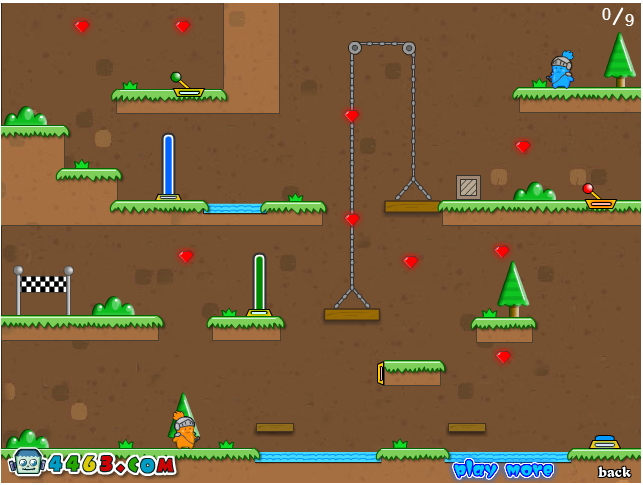
\includegraphics[width=.60\textwidth]{./imagenes/gatos1.png}
\caption{Gatos Gemelos}
\label{Gatos Gemelos}
\end{center}
\end{figure}
Gatos Gemelos \footnote{\url{http://ar.yayoye.com/twin-cat-online-game/22643/}} es un Juego en el que se deben mover a los personajes por la pantalla, como su nombre mismo lo dice son unos gatos gemelos, con los que iremos tratando de recoger diamantes y de lograr que interactúen entre ellos para superar los obstáculos.

\subsubsection{¿Por qué es uno de mis juegos favoritos?}
\begin{itemize}
\item[Tania Sánchez] En realidad no soy de esas personas que se vician con los juegos pero me llaman mucho la atención el tipo de juego que estimula el aprendizaje, me parece que este juego lo hace, ya que es un juego que se realiza en pareja en el que enseña el trabajo en equipo, a medida que avanzan los niveles va aumentando la dificultad del mismo, poniendo al usuario cada vez a pensar más en como vencer los obstaculos tomando en cuenta que un jugador debe ir a la par con el otro e irlo ayudando para juntos llegar a la meta, la dificultad del juego aparte de resolver como se debe avanzar, está en no olvidarse del compañero ya que aunque llegue uno de los dos solo a la meta no implicará que se pasará al siguiente nivel sino que deben llegar los dos juntos. 
\\
\\
Éste es un juego orientado más para niños pequeños para estimular el desarrollo intelectual y enseñarles el trabajo en equipo =).
\end{itemize}


\chapter{Conclusiones}
Cuales juegos fueron más populares y un breve razonamiento del porqué.

\end{document}  
